Bei einer Welle reicht \emph{ein} Diagramm zur Darstellung nicht aus. Da es mehrere Oszillatoren gibt, die alle zu unterschiedlichen Zeiten zu schwingen beginnen, bräuchte man ein Elongation-Zeit-Diagramm (\referenz{sec:diagramm_schwingung}) für jedes Teilchen, oder ein 3-dimensionales Diagramm, um die Schwingung aller Teilchen in Abhängigkeit \emph{eines} Zeitpunktes darzustellen.

Allerdings reichen zwei Diagramme um alle Kenngrößen der Welle erfassen und ablesen zu können: Ein Elongation-Zeit-Diagramm eines beliebigen Teilchens, welches die Schwingung dieses Teilchens über der Zeit darstellt und ein Elongation-Strecke-Diagramm (ein \glqq Standbild\grqq) zu einem beliebigen Zeitpunkt, welches die Auslenkung der Oszillatoren über der x-Position dieser Oszillatoren darstellt.

\begin{figure}[h!]
	\centering
	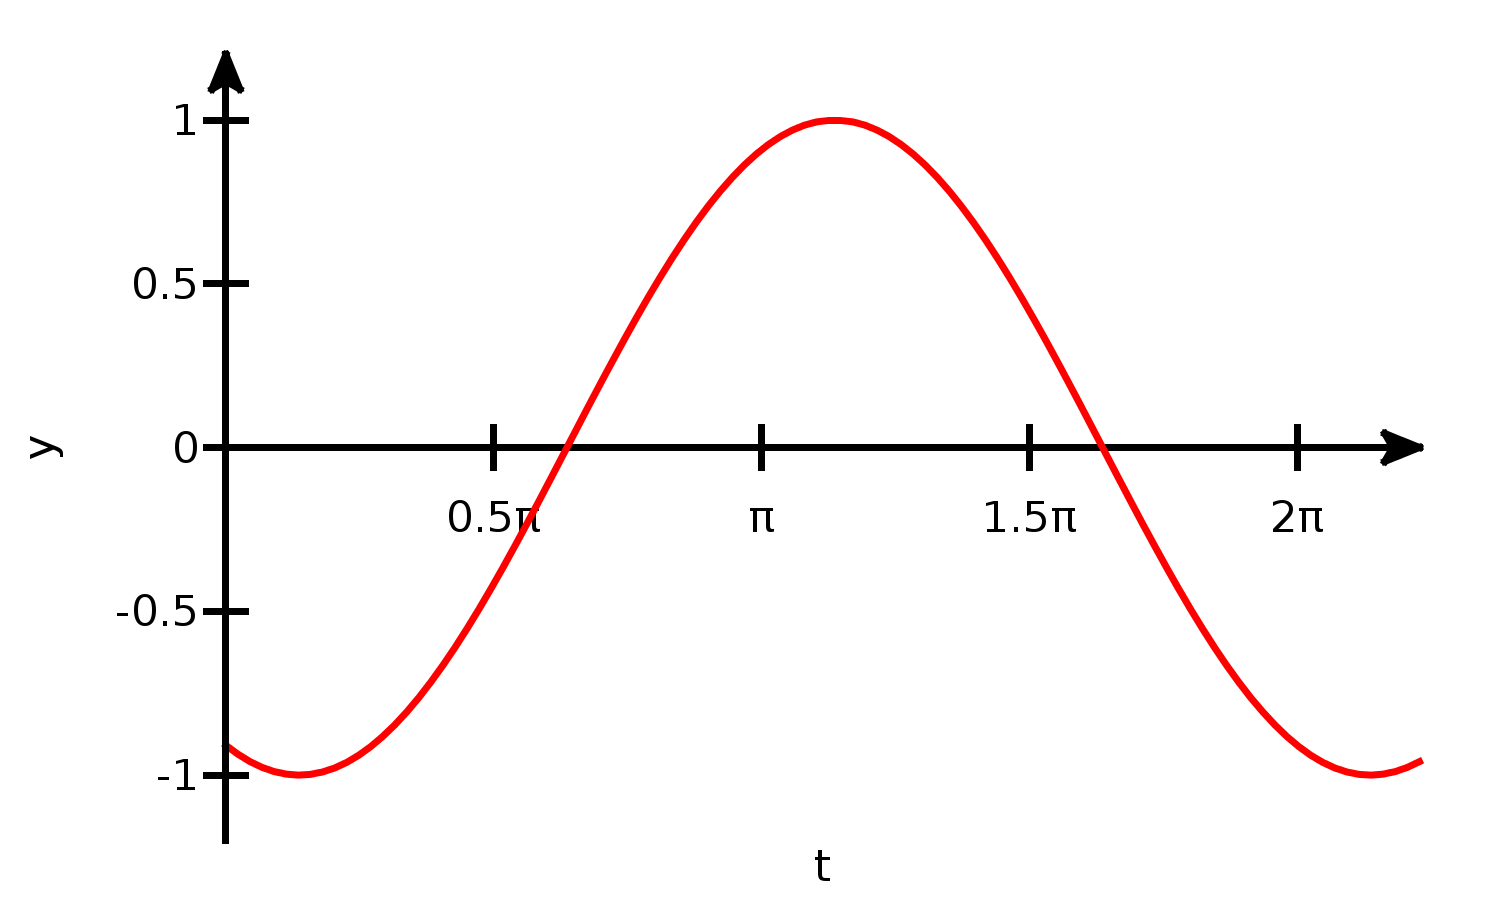
\includegraphics[width=0.9\textwidth]{welle_bei_x}
	\begin{comment} 'plot_pitics.p'
set dummy t
set ylabel "y"
set xlabel "t"
unset key
set output 'welle_bei_x.png'
plot sin(2*pi*((t/(2*pi))-(1/pi))) ls 1
	\end{comment}
	\caption{Elongation-Zeit-Diagramm des Teilchens mit Abstand $x=1$ zum Ursprung.}
	\label{fig:welle_bei_x}
\end{figure}
\begin{figure}[h!]
	\centering
	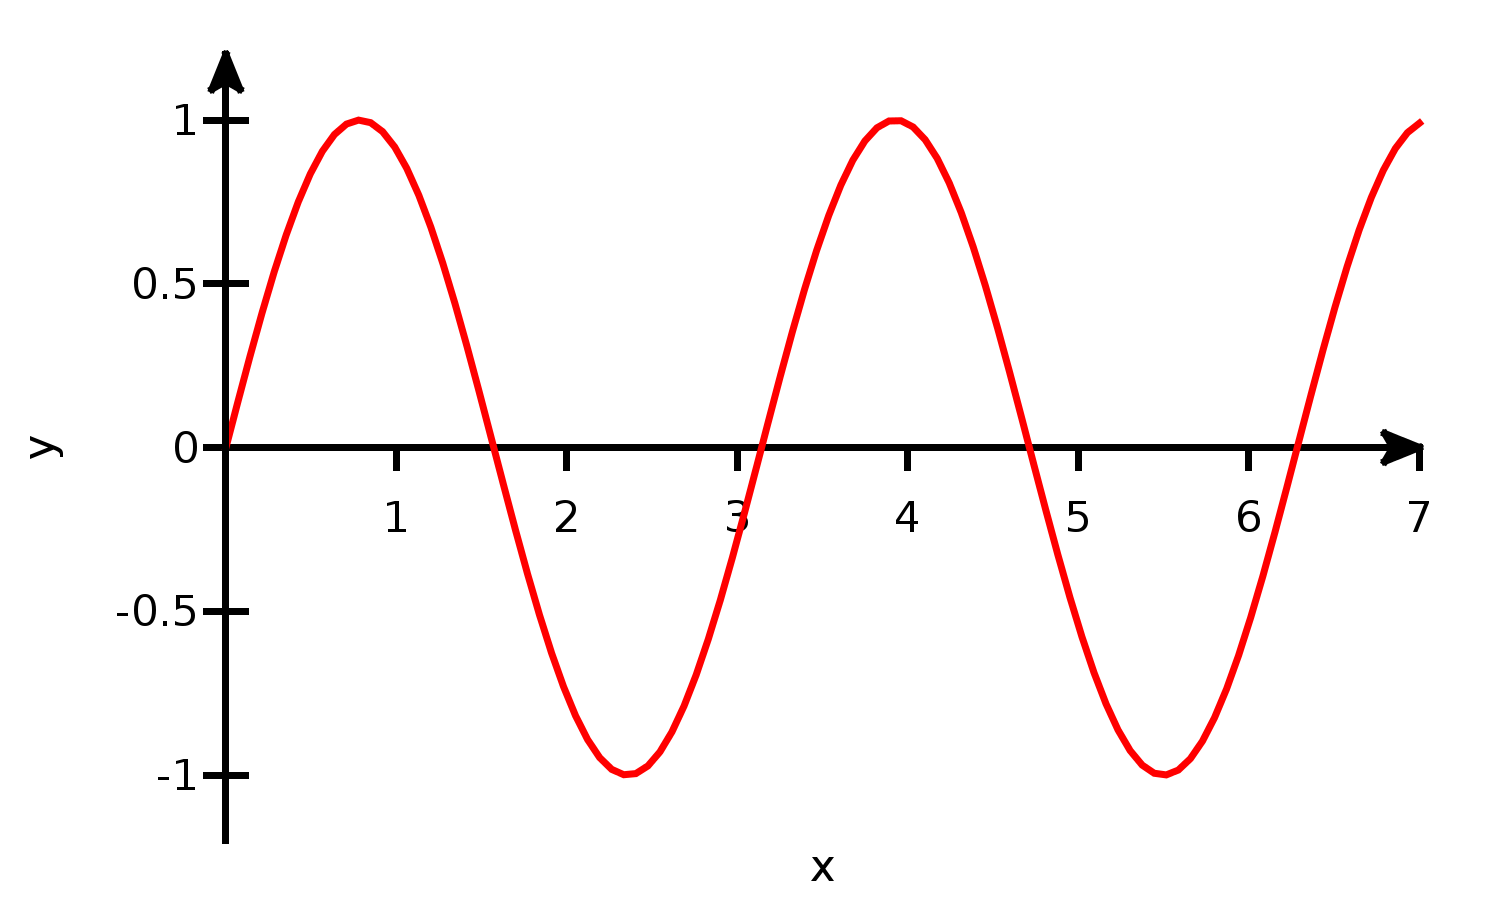
\includegraphics[width=0.9\textwidth]{welle_zu_t}
	\begin{comment} 'plot_pitics.p'
set dummy x
set ylabel "y"
set xlabel "x"
unset xtics
set xtics axis
set xtics ('1' 1, '2' 2, '3' 3, '4' 4, '5' 5, '6' 6, '7' 7)
set xzeroaxis ls 2
unset key
set output 'welle_zu_t.png'
plot sin(2*pi*((pi/(2*pi))-(x/pi))) ls 1
	\end{comment}
	\caption{Elongation-Abstand-Diagramm (\glqq Standbild\grqq ) zum Zeitpunkt $t=\pi$}
	\label{fig:welle_zu_t}
\end{figure}

Dazu muss angemerkt werden, dass hierbei nur eine Dimension betrachtet wird, eigentlich müsste die komplette räumliche Ausbreitung bei einem Elongation-Strecke-Diagramm berücksichtigt werden, in alle 3 Dimensionen. Zur Vereinfachung, damit man statt einem 4-Dimensionalen Diagramm ein 2-Dimensionales (x,y) Diagramm benutzen, wird nur \emph{eine} Ausbreitungsrichtung berücksichtigt.
